

\section{LEGO-GraphRAG Framework}
\label{section: Modular GraphRAG}

%To demonstrate the functionalities of our framework, we focus on its retrieval phase of GraphRAG, one of its two primary phases, as it provides the essential reasoning information required for subsequent augmentation and generation in LLMs. To deepen understanding of this key phase, we introduce the LEGO-GraphRAG framework, which organizes the retrieval process into two modular components with workflow-dependent module configurations. For each module, we systematically categorize and summarize the available methods, rendering the framework's design solutions.


\subsection{Overview}
Table~\ref{tab:design-space} outlines the design framework of LEGO-GraphRAG, structured along two key dimensions: {\bf modules} and {\bf method types}. Specifically, the core retrieval phase is divided into two modules: the \textit{subgraph-extraction} module and the \textit{path-retrieval} module. Each module incorporates two solution types: \textit{structure-based} methods and \textit{semantic-augmented} methods.
Accordingly, GraphRAG instan\\ces within the LEGO-GraphRAG framework are classified into five distinct groups based on the combinations of modules and solution types used.  
Table~\ref{tab:flat_table} provides a detailed breakdown of these groups, encompassing both existing methods and new instances developed in our empirical study.
In general, the LEGO-GraphRAG framework is materialized by two key considerations.
\begin{itemize}[leftmargin=10pt]
    \item {\bf Natural Segmentation of the GraphRAG Process.} 
    %Facilitating a natural segmentation of the GraphRAG process, wherein the reasoning path retrieval consists of: 
    The reasoning path retrieval process is naturally segmented into two phases:
    a) extracting a query-relevant subgraph to scale down the search space; and b) meticulously retrieving reasoning paths from the extracted subgraph.
    \item %Facilitating the analysis of recent advancements in GraphRAG research: 
    {\bf Facilitation of GraphRAG Research Analysis.} 
    %A review of current developments in GraphRAG reveals that most contributions can be categorized as improvements to one or both of the two modules, 
    The framework enables a comprehensive analysis of recent GraphRAG advancements, which predominantly focus on enhancing one or both modules, as summarized in Table~\ref{tab:flat_table}. 
\end{itemize}

\vspace{-5pt}
\subsubsection{{\bf {\PreRetrieval} {\bf vs.} {\Retrieval} Modules}}

%{\color{red}The design of these two modules is driven by two key considerations.}

The subgraph-extraction (SE) module aims to enhance the effectiveness and efficiency of reasoning path retrieval by reducing the search space from the full graph to a smaller set of query-relevant subgraphs. The path-retrieve (PR) module then operates on these subgraphs to retrieve reasoning paths using specific methods. 
%For the module of subgraph-extraction (SE {\it in short}), the main goal is to improve both the effectiveness and efficiency of the subsequent retrieval of reasoning paths. This is achieved by scaling down the search space from the entire graph to a set of small-scale subgraphs which are query-relevant.
%The function of the path-filtering (PF {\it in short}) module is to retrieve reasoning paths from the previously extracted query-relevant subgraphs using specific methods.
Based on the retrieval phase of GraphRAG formalized in Definition~\ref{def:retrieval}, the two modules are formalized as follows.

\begin{definition}[\textbf{\PreRetrieval ~(\ShortPreRetrieval)}]
\label{def:pf}
\vspace{-5pt}
Given a query $q$, a graph $G = (V, E)$, and a set of entities and relations $\epsilon_q$ derived from specified query $q$, the SE module aims to extract a query-specific subgraph $g_q \subseteq G$, defined as:~~~~
$\ShortPreRetrieval(G, q, \epsilon_q) \rightarrow g_q$.
%The subgraph extraction process can therefore be formalized as: 
%\begin{equation} 
%\small
%	\ShortPreRetrieval(G, q, \epsilon_q) \rightarrow g_q 
%    \vspace{-5pt}
%\end{equation}
\end{definition}



\begin{definition}[\textbf{\Retrieval~(\ShortRetrieval)}]
\vspace{-5pt}
Given an extracted subgraph $g_q \subseteq G$ and the entity and relation set $\epsilon_q$ derived from query $q$, the process of this module obtains a reasoning path set $\mathcal{P}_q = \{P_i^{(q)}\}$ with the following process:~~~~ $\ShortRetrieval(G\text{~or~} g_q, q, \epsilon_q)  \rightarrow \mathcal{P}_q = \{P_i^{(q)}\}$.
%\begin{equation}
%\small
% \ShortRetrieval(G\text{~or~} g_q, q, \epsilon_q)  \rightarrow \mathcal{P}_q = \{P_i^{(q)}\} %\rightarrow 
%\end{equation}
\end{definition}


\begin{table*}[h]
	\caption{Design Solutions of LEGO-GraphRAG Framework: \it{\small The framework comprises of four groups of instances: (I) SBE \& SBR; (II) SBE \& I/OSAR; (III) SAE \& SBR; (IV) SAE \& I/OSAR. 
 When the subgraph-extraction module is optional, an additional group, (V) SBR or I/OSAR, is included.}}
    \vspace{-65pt}
	\label{tab:design-space}
	\resizebox{\textwidth}{!}{%
		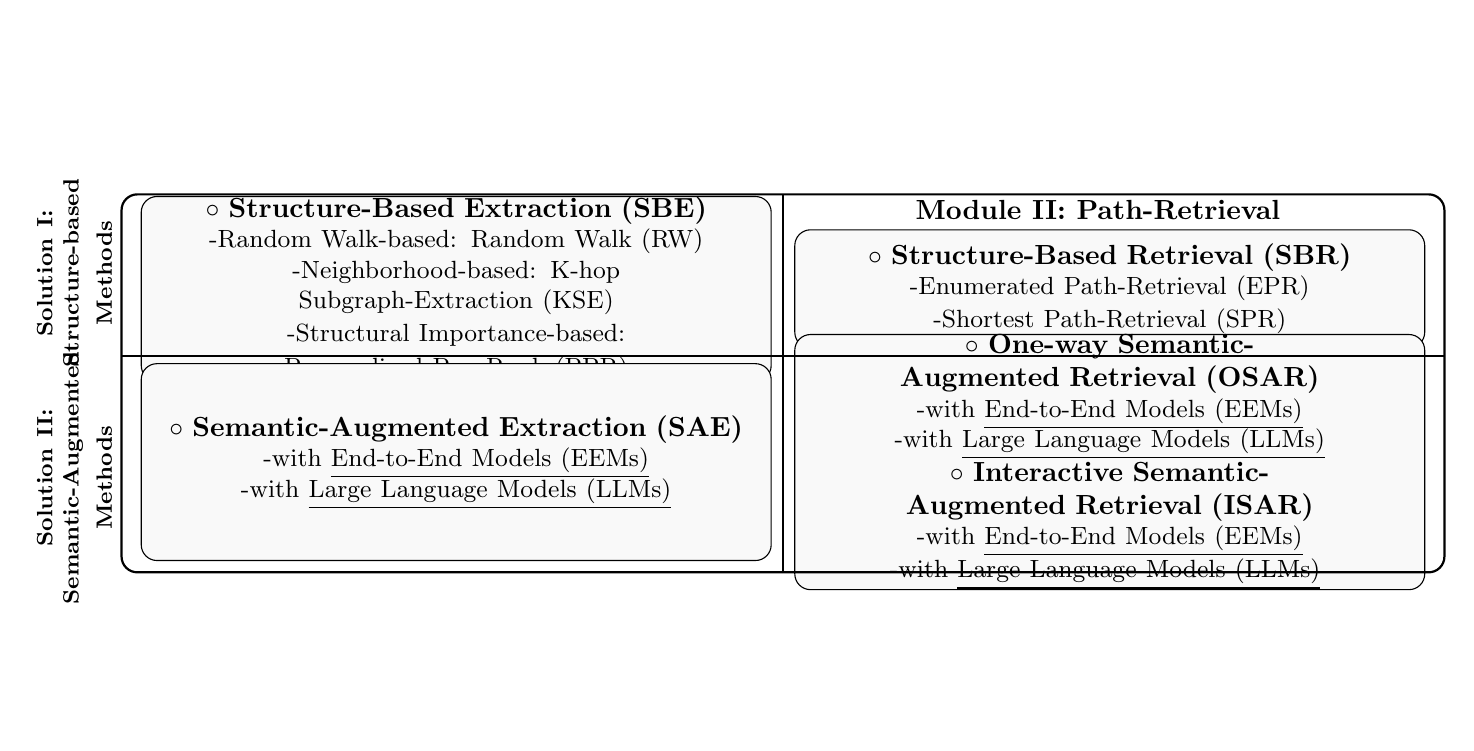
\begin{tikzpicture}
			\tikzstyle{block} = [draw, rounded corners=2mm, thin, minimum width=8cm, minimum height=2.5cm, align=center, inner sep=0pt, text width=8cm, fill=gray!5]

              \tikzstyle{block2} = [draw, rounded corners=2mm, thin, minimum width=8cm, minimum height=1.5cm, align=center, inner sep=0pt, text width=8cm, fill=gray!5]
			\tikzstyle{title} = [align=center, font=\bfseries, text width=8cm]
			\tikzstyle{vtitle} = [align=center, font=\bfseries, rotate=90, anchor=center, text width=6cm]
			% Horizontal Titles
			\node[title] (title1) at (-8.2, 5) { \textsc{Module I: Subgraph-Extraction}};
			\node[title] (title2) at (0, 5) { \textsc{Module II: Path-Retrieval}};
			% Vertical Titles
			\node[vtitle] (title3) at (-13, 4.2) { \textsc{\footnotesize Solution I: \\Structure-based \\Methods}};
			\node[vtitle] (title4) at (-13, 1.6) { \textsc{\footnotesize Solution II: \\Semantic-Augmented \\Methods}};
			
			% Top Left Block
			\node[block2] (block1) at (-8.15, 4) {
				{\bf $\circ$ Structure-Based Extraction (SBE)} \\ 
                {\small
                    -\text{Random Walk-based: Random Walk (RW)}\\
                    -\text{Neighborhood-based: K-hop Subgraph-Extraction (KSE)} \\
				-\text{Structural Importance-based: Personalized PageRank (PPR)} }\\
			};
			
			% Top Right Block
			\node[block2] (block2) at (0.15, 4) {
				{\bf $\circ$  Structure-Based  Retrieval (SBR)} \\ 
                {\small
				-\text{Enumerated Path-Retrieval (EPR)} \\
                    -\text{Shortest Path-Retrieval (SPR)} 
                    }
			};
			
			% Bottom Left BlockPath
			\node[block] (block3) at (-8.15, 1.8) {
				{\bf $\circ$ Semantic-Augmented Extraction  (SAE)} \\ 
                {\small
				-\text{with \underline{End-to-End Models (EEMs)}}\\
                -\text{with \underline{Large Language Models (LLMs)} } \\ 
                }
			};
			
			% Bottom Right Block
			\node[block] (block4) at (0.15, 1.8) {
				{\bf $\circ$ One-way Semantic-Augmented Retrieval (OSAR)} \\ 
                {\small
			-\text{with \underline{End-to-End Models (EEMs)}} \\
            -\text{with \underline{Large Language Models (LLMs)} }\\
            }
				{\bf $\circ$ Interactive Semantic-Augmented Retrieval (ISAR)} \\ 
		      {\small
            -\text{with \underline{End-to-End Models (EEMs)}}\\
            -\text{with \underline{Large Language Models (LLMs)} }
            }
            \\ };
			
			% Large Rounded Rectangle Enclosing All Four Blocks
			\draw[rounded corners=2mm, thick] 
			(-12.4, 0.4) rectangle (4.4, 5.2);
			
			% Horizontal Line in the Center
			\draw[thick] (-12.4, 3.15) -- (4.4, 3.15);
		
			% Vertical Line in the Center
			\draw[thick] (-4, 0.39) -- (-4, 5.2);
		\end{tikzpicture}
        	}
            
            \vspace{-60pt}           
\end{table*}





% Please add the following required packages to your document preamble:
% \usepackage{graphicx}

% Please add the following required packages to your document preamble:
% \usepackage{multirow}
% \usepackage{graphicx}

% Please add the following required packages to your document preamble:
% \usepackage{multirow}
% \usepackage{graphicx}

% Please add the following required packages to your document preamble:
% \usepackage{multirow}
% \usepackage{graphicx}


\begin{table*}[]
    \footnotesize
        \caption{Five Groups of Instances under the LEGO-GraphRAG Framework}
        \vspace{-10pt}
        \label{tab:flat_table}
        %\renewcommand{\arraystretch}{1}
        \resizebox{\textwidth}{!}{%
        \begin{tabular}{
            >{\centering\arraybackslash}m{2.5cm} % 第一列
            >{\centering\arraybackslash}m{2.5cm} % 第二列
            >{\centering\arraybackslash}m{3cm}   % 第三列
            >{\centering\arraybackslash}m{3cm}   % 第四列
            >{\centering\arraybackslash}m{4cm}   % 第五列（原第六列）
        }
        \hline
        \multicolumn{2}{c}{\textbf{Group}} &
          \textbf{\makecell{Subgraph-Extraction}} &
          \textbf{\makecell{Path-Retrieval}} &
          \textbf{\makecell{Implemented Instances}} \\ 
        \hline
        \multicolumn{2}{c}{\textbf{\makecell{Structure-based Methods on Both \\Modules (Group (I): {\it SBE \& SBR}) }}} &
          SBE (-RW/KSE/PPR) &
          SBR (-EPR/SPR) &
          Our Instance: No.{\PPRxSPR} \\ 
        \hline
        \multicolumn{2}{c}{\multirow{2}{*}{\textbf{\makecell{Semantic-Augmented Methods\\ on Both Modules \\ (Group (II): {\it SAE \& I/OSAR})}}}} &
          SAE (-EEMs/LLMs) &
          OSAR (-EEMs/LLMs) &
          \makecell{Our Instances: No.{\EEMxEEMxOSAR}, {\EEMxLLMxOSAR}, {\LLMxEEMxOSAR}, {\LLMxLLMxOSAR}} \\ \cline{3-5} 
        \multicolumn{2}{c}{} &
          SAE (-EEMs/LLMs) &
          ISAR (-EEMs/LLMs) &
          \makecell{GCR (arXiv24)~\cite{GCR} \\ Our Instances: No.{\EEMxEEMxISAR}, {\EEMxLLMxISAR}, {\LLMxEEMxISAR}, {\LLMxLLMxISAR}} \\ 
        \hline
        \multicolumn{2}{c}{\textbf{\makecell{Semantic-Augmented Methods\\ on Subgraph-Extraction \\(Group (III): {\it SAE \& SBR})}}} &
          SAE (-EEMs/LLMs) &
          SBR (-EPR/SPR) &
          \makecell{RoG (ICLR24)~\cite{RoG} \\ GSR (EMNLP24)~\cite{LessIsMore} \\ Our Instances: No.{\EEMxSPR}, {\LLMxSPR}} \\ 
        \hline
        \multicolumn{2}{c}{\multirow{2}{*}{\textbf{\makecell{Semantic-Augmented Methods\\ on Path-Retrieval \\ (Group (IV): {\it SBE \& I/OSAR})}}}} &
          SBE (-RW/KSE/PPR) &
          OSAR (-EEMs/LLMs) &
          \makecell{Our Instances: No.{\PPRxEEMxOSAR}, {\PPRxLLMxOSAR}} \\ \cline{3-5} 
        \multicolumn{2}{c}{} &
          SBE (-RW/KSE/PPR) &
          ISAR (-EEMs/LLMs) &
          \makecell{StructGPT (EMNLP23)~\cite{StructGPT} \\ Our Instances: No.{\PPRxEEMxISAR}, {\PPRxLLMxISAR}} \\ 
        \hline
            \multicolumn{2}{c}{\multirow{3}{*}{\textbf{\makecell{Without Subgraph-Extraction \\ Modules \\(Group (V): {\it SBR or I/OSAR})} }}} &
          None &
          SBR (-EPR/SPR) & -
           \\ \cline{3-5} 
        \multicolumn{2}{c}{} &
          None &
          OSAR (-EEMs/LLMs) &
          \makecell{KELP (ACL24)~\cite{ref:kelp}} \\ \cline{3-5} 
        \multicolumn{2}{c}{} &
          None &
          ISAR (-EEMs/LLMs) &
          \makecell{ToG (ICLR24)~\cite{ToG}, DoG (arXiv24)~\cite{DoG}} \\ 
        \hline
        \end{tabular}%
        \vspace{-10pt}
        }
        %\vspace{-10pt}
    \end{table*}

\begin{comment}


\begin{table*}[ht]
    \centering
    \caption{Flat Table of Subgraph Extraction and Path Retrieval Combinations}
    \label{tab:flat_table}
    \begin{tabular*}{\textwidth}{@{\extracolsep{\fill}}lccccc@{}}
        \toprule
        \textbf{ID} & \textbf{Group} & \textbf{Subgraph-Extraction} & \textbf{Path-Retrieval} & \textbf{Semantic Enhancement} & \textbf{Implemented Instances} \\
        \midrule
        \multicolumn{6}{c}{\textbf{No Subgraph Extraction}} \\
        \midrule
        1  & SBE+SBR   & None            & ISER (-LLMs)   & None & StructGPT (EMNLP23)~\cite{StructGPT} \\
        2  & SBE+OSER  & None            & OSER (-EEMs/LLMs) & Path-Retrieval & ToG (ICLR24)~\cite{ToG} \\
        3  & SBE+OSER  & None            & OSER (-EEMs)   & Path-Retrieval & KELP (ACL24)~\cite{ref:kelp} \\
        4  & SBE+ISER  & None            & ISER (-LLMs)   & Path-Retrieval & DoG (arXiv24)~\cite{DoG} \\
        \midrule
        \multicolumn{6}{c}{\textbf{Semantic Enhancement on Both Modules}} \\
        \midrule
        5  & SEE+OSER  & PPR+ST         & SPR+ST         & Both & GSR (arXiv24)~\cite{LessIsMore} \\
        6  & SEE+OSER  & PPR+ST         & SPR+LLM        & Both & GCR (arXiv24)~\cite{GCR} \\
        7  & SEE+OSER  & PPR+LLM        & SPR+ST         & Both & - \\
        8  & SEE+OSER  & PPR+LLM        & SPR+LLM        & Both & - \\
        \midrule
        \multicolumn{6}{c}{\textbf{Semantic Enhancement on Subgraph-Extraction}} \\
        \midrule
        9  & SEE+SBR   & SEE (-LLMs)     & SBR            & Subgraph-Extraction & RoG (ICLR24)~\cite{RoG} \\
        10 & SEE+SBR   & PPR+ST         & SPR            & Subgraph-Extraction & - \\
        11 & SEE+SBR   & PPR+LLM        & SPR            & Subgraph-Extraction & - \\
        \midrule
        \multicolumn{6}{c}{\textbf{Semantic Enhancement on Path-Retrieval}} \\
        \midrule
        12 & SBE+OSER  & PPR            & SPR+ST         & Path-Retrieval & - \\
        13 & SBE+OSER  & PPR            & SPR+LLM        & Path-Retrieval & - \\
        14 & SBE+ISER  & PPR            & BS+ST          & Path-Retrieval & - \\
        15 & SBE+ISER  & PPR            & BS+LLM         & Path-Retrieval & - \\
        \bottomrule
    \end{tabular*}
\end{table*}



\end{comment}



\vspace{-5pt}
Of the two modules, the {\it \retrieval} module is essential for any GraphRAG instance, while the {\it \preRetrieval} module is optional.
The optionality of the {\it \preRetrieval} module depends largely on the graph size, primarily due to computational efficiency. 
For smaller graphs, where the node and edge space remain manageable, direct retrieval of reasoning paths is feasible, making the {\it \preRetrieval} module optional. 
However, for large-scale graphs, the exponential growth in the number of nodes, edges, and paths significantly complicates the retrieval {\cite{BigGraphVLDB,PrismX,SummaryBigGraph,SysBigGraph}}. 
The {\it \preRetrieval} module addresses this by extracting a query-relevant subgraph, reducing the retrieval space and improving computational efficiency and relevance.
After passing through these modules, the refined reasoning paths enhance the reasoning abilities of LLMs during the generation phase, as detailed in Definition~\ref{def:generation}.


\vspace{-5pt}
\subsubsection{\bf Structure-based {\bf vs.} Semantic-augmented Methods}


For each module, systematically classifying and summarizing potential solutions is important, as it enables the identification of potential strategies and provides a deeper understanding of existing implementations.  
At their core, the workflows of the {\it \preRetrieval} and {\it \retrieval} modules share potential similarities, as both involve 
retrieving a small-scale but query-relevant subset from the graph.
%``retrieval'' processes aiming at extracting a smaller but query-relevant subset from a large graph. 
Accordingly, the design solutions for these modules can be interwoven and further categorized into two complementary categories: {\it structure-based methods}, focusing on the graph's topological properties, and {\it semantic-augmented methods}, utilizing the semantic information of both the graph and the query, as detailed in Table~\ref{tab:design-space}.

%{\bf ([cites] Papers on Survey of graph algorithms, especially graph walk algorithms in SIGMOD, VLDB, XXX)}
Structure-based methods (SBE and SBR) use graph algorithms~\cite{Korf1985DepthFirstIA,ThunderRW,FastRWR,FastPPR,Topppr,PPRSurvey} to iteratively explore nodes (entities) and edges (relations), %connected to query entities, thereby 
constructing subgraphs or reasoning paths.
Semantic-augmented methods (SAE, OSAR, and ISAR) exploit the semantic relevance between the query and the nodes, edges, and triples of graphs, using two types of semantic models: end-to-end models (EEMs) {\cite{reimers-2019-sentence-bert,reimers-2020-multilingual-sentence-bert,thakur-2020-AugSBERT}} and large language models (LLMs) {\cite{LLMSurvey,ToG,GraphInsight}}. 
The two types of models are applied differently. 
%can be utilized in different ways. 
%Methods including SAE and OSAR employ models of EEMs or LLMs to refine candidate subgraphs or reasoning paths, getting better alignment with the query's semantics. 
SAE/OSAR methods refine candidate subgraphs/paths for better semantic alignment.
ISAR methods incorporate semantic evaluation directly into the path-retrieval process, using EEMs/LLMs to interactively identify relevant reasoning paths.
In the sequel, we investigate the design solutions of the two modules, subgraph-extraction (Section~\ref{subsection: design solutions of preretrieval}) and path-retrieval (Section~\ref{subsection: design solutions of retrieval}), with the aforementioned two types of methods, structure-based and semantic-augmented methods.
%\input{tables/ref.tex}

\vspace{-5pt}
\subsection{Design Solutions of {\PreRetrieval}}
\label{subsection: design solutions of preretrieval}

The design solution of the subgraph-extraction module is comprised of \textit{structure-based extraction} (\textbf{SBE} in Section~\ref{subsec:sbe}) and \textit{semantic-based extraction} (\textbf{SAE} in Section~\ref{subsec:sae}).

\vspace{-5pt}
\subsubsection{{\bf Structure-Based Extraction ({\bf SBE})}} 
\label{subsec:sbe}
These solutions exploit the structural information of a graph \( G = (V, E) \), starting with the query-relevant entities \( \{v_i^{(q)}\} \in \epsilon_q \),\footnote{While subgraphs can be built from relationship \( e_i^{(q)} \in \epsilon_q \), practical methods predominantly use entities (nodes) as the basis for subgraph construction~\cite{ref:kelp,ToG,ChatKBQA,GCR,LessIsMore}.} to identify corresponding nodes (entities) and edges (relations) that are pertinent to the query \( q \). This process constructs smaller subgraphs centered around each \( v_i^{(q)} \), which are then aggregated to produce the query-related subgraph \( g_q \). Formally, the procedure is defined as:
\begin{equation*}
\small
\ShortPreRetrieval(G, q, \epsilon_q) \rightarrow g_q = \bigcup\nolimits_{v_i^{(q)} \in \epsilon_q} g_{(q,v_i^{(q)})}
\vspace{-5pt}
\end{equation*}

Here, \( g_q \) represents the union of the subgraphs \(g_{(q,v_i^{(q)})} \), each focusing on an entity \( v_i^{(q)} \) in \( \epsilon_q \). For each query entity, three extraction strategies can be applied: {\it random walk-based}, {\it neighborhood-based}, and {\it structural importance-based} strategies.

{\it \underline{a) Random Walk-based.}} The {\it random walk (RW)} algorithm {\cite{RandomWalk,kRW}} and its variants {\cite{LRW,RWR,FastRWR,SecondRW,SpaceRW} enumerate all entities in $\epsilon_q$, and, for each entity $v_i^{(q)}$,
%can start from an entity \( v_i^{(q)} \) and 
iteratively expand a subgraph by randomly selecting edges and nodes at each step. This simple yet effective strategy gradually constructs a subgraph of the desired size, making it a commonly used baseline method~\cite{NSM,RoG,LessIsMore,GCR}.

{\it \underline{b) Neighborhood-based.}} This strategy aims to capture the local structure around an entity \( v_i^{(q)}\in \epsilon_q \) by expanding its neighborhood. The most representative method is {\it K-hop subgraph-extraction (KSE)} {\cite{NSM}}, where the subgraph is constructed by including all nodes \( v_j \) and edges \( e_{ij} \) such that the shortest path distance \( d(v_i^{(q)}, v_j) \leq K \). 
This approach ensures that the subgraph captures the immediate relational context surrounding the query entity, progressively including nodes and edges within the specified radius (i.e., $K$-hops).



{\it \underline{c) Structural Importance-based.}} These methods  {\cite{PageRank,PPR,PPRSurvey}} identify nodes based on their structural importance relative to an entity \( v_i^{(q)} \). Nodes are ranked by importance scores, and a subset of high-ranking $N_{ppr}$ nodes, along with their directly connected edges, are selected to form the subgraph.
Prominent methods, such as {\it PageRank} {\cite{PageRank}} and {\it Personalized PageRank (PPR)} {\cite{PPR}}, compute a relevance score for each node based on topological position, link density and centrality.
Specifically, PageRank assigns an importance score \( S(v_j) \) to each node \( v_j \), which is iteratively updated based on both its local connectivity and the scores of its neighboring nodes, thereby capturing its global significance. Personalized PageRank (PPR) enhances this process by ``personalizing'' the distribution towards the query entity \( v_i^{(q)} \), ensuring that nodes closer to \( v_i^{(q)} \) receive higher scores.
%\footnote{Formally, given a \( v_i^{(q)} \), the PPR score for each node \( v_j \) is computed as \( S(v_j) = \alpha \cdot \delta(v_j, v_i^{(q)}) + (1-\alpha) \sum_{(v_k,v_j) \in E} \frac{S(v_k)}{\deg(v_k)} \), where \(\alpha\) is the restart probability, \(\delta(v_j, v_i^{(q)}) = 1\) if \( v_j = v_i^{(q)} \) and 0 otherwise, and \(\deg(v_k)\) is the out-degree of \(v_k\). The equation is solved iteratively until convergence.} 
While PPR is a widely adopted approach for SBE solutions, its computational cost scales with the size of the graph, presenting a considerable bottleneck for real-time GraphRAG pipelines. Section~\ref{exp:PreRetrieval} discusses this efficiency challenge in detail.




%{\color{red}Formally, given a query entity \( v_i^{(q)} \), the PPR score \( S(v_j) \) for each node \( v_j \) can be computed as:
%\(
%S(v_j) = \alpha \cdot \delta(v_j, v_i^{(q)}) + (1-\alpha) \sum_{(v_k,v_j) \in E} \frac{S(v_k)}{\deg(v_k)},
%\)
%where \(\alpha\) is the restart probability, \(\delta(v_j, v_i^{(q)})=1\) if \( v_j = v_i^{(q)} \) and 0 otherwise, and \(\deg(v_k)\) is the out-degree of \(v_k\). This equation is typically solved through iterative updates, repeatedly redistributing scores until they converge to a stable solution.}

\vspace{-5pt}
\subsubsection{{\bf Semantic-Augmented Extraction ({\bf SAE})}}
\label{subsec:sae}
%These solutions integrates semantic information to facilitate subgraph extraction by evaluating the semantic relevance of nodes and edges with respect to the query. Semantic relevance is typically assessed using semantic models, which classify methods into two main categories: those based on \textit{end-to-end models (EEMs)} and those based on \textit{large language models (LLMs)}.
%Solutions that integrate semantic information to facilitate subgraph extraction typically evaluate semantic relevance using semantic models. 
Semantic models play a key role in facilitating subgraph-extraction by assessing the semantic relevance of graph components.
These models fall into two main categories: %those based on 
End-to-End Models (EEMs) and Large Language Models (LLMs).


{\it \underline{a) End-to-End Models (EEMs).}} 
%EEMs typically take the text of graph components 
EEMs process the text associated with graph components 
(i.e., nodes, edges, triples) and queries to compute semantic relevance.
They either output statistical properties and embeddings for relevance calculation or directly provide relevance scores.
%as input, and either output statistical semantic properties and embedding vectors for calculating relevance scores, or directly output relevance scores.
Formally, for nodes, edges, or triples \( v, e, \text{~or~} \tau \in G \) and a query \( q \), the goal is: $\text{EEMs} (v \text{ or } e \text{ or } \tau, q) \to \text{scores}.$ 
%\begin{equation}
%\small
%\label{eq:EEMs_score}
%\text{EEMs} (v \text{ or } e \text{ or } \tau, q) \to \text{scores}.
%\end{equation}
Using these scores, the most relevant graph components are identified for subgraph-extraction.
%Based on the relevance score derived from the EEMs, the most relevant nodes and edges for subgraph extraction can be identified. Next, we introduce the typical types of models within EEMs and their mechanisms, followed by a detailed description of the general workflow for subgraph extraction using EEMs.
EEM can be categorized into two main types: {\it Statistical Models} {\cite{TFIDF,BM25,BM25+}} and {\it Embedding Models/Re-Rankers} {\cite{reimers-2019-sentence-bert,BGE}}. The former relies on statistical computations, while the latter consists of end-to-end neural network models to produce embeddings or rank relevance. 



%\begin{itemize}[leftmargin=10pt]
   %\item 
   {\it \uwave{a).1 Statistical Models.}}
Statistical models are foundational in text analysis and semantic modeling, relying on metrics 
%which  evaluates semantic similarity based on statistical properties 
like term frequency (TF) and inverse document frequency (IDF)  {\cite{TFIDF}}. 
Popular methods include {\it BM25}  {\cite{BM25}} for ranking relevance in information retrieval, {\it Latent Semantic Analysis (LSA)}  {\cite{LSA}}  for uncovering latent semantic structures via dimensionality reduction, and {\it Latent Dirichlet Allocation (LDA)}  {\cite{LDA}}  for topic modeling, which aids 
%can indirectly aid 
semantic similarity through topic distributions.


For example, BM25 treats textual information attached to graph components (nodes, edges, or triples) as ``documents'' within a corpus (the graph). 
During precomputation, the text of each graph component is tokenized, enabling the calculation of TF and IDF. 
When a query is issued, its text undergoes tokenization, 
and BM25 computes a relevance score for each graph component based on the query terms and their frequency distributions across the graph. 
%the relevance score using:
%resulting in comparable TF and IDF statistics. 
%Using these properties, BM25 computes relevance scores between the query and graph components by quantifying the frequency and importance of ``best matches'':
%\begin{equation}
%\footnotesize
%\text{BM25}(v, q) \to \sum_{t \in \text{Tk}(q)} IDF(t) \cdot \frac{TF(t, \text{Tk}(v)) \cdot (k_1 + 1)}{TF(t, \text{Tk}(v)) + k_1 \cdot (1 - b + \frac{b \cdot |\text{Tk}(v)|}{\text{avglen}})} ~\footnote{Here, \( t \) is a token from the tokenized query \( \text{Tk}(q) \), \( TF(t, \text{Tk}(v)) \) is the term frequency of \( t \) in \( v \)'s tokenized text, and \( IDF(t) = \log \frac{N - n_t + 0.5}{n_t + 0.5} \), where \( N \) is the total number of documents and \( n_t \) is the number of documents containing \( t \). \( \text{avglen} \) is the average tokenized document length in the corpus, \( |\text{Tk}(v)| \) is the length of \( v \)'s tokenized text, and \( k_1 \), \( b \) are hyperparameters.}
%\end{equation} 
Statistical models are efficient, with low computational costs and short execution times. They are suitable for simpler semantic tasks or as baselines in semantic-augmented workflows.


%{\color{red} {\bf Make detailed explanation in footnotes.}\( TF(t, \text{tokens}(v)) \) is the term frequency of \( t \) in the tokenized text of \( v \); \( IDF(t) \) is the inverse document frequency of \( t \), calculated as \( \log \frac{N - n_t + 0.5}{n_t + 0.5} \), with \( N \) being the total number of documents (graph components) in the corpus, and \( n_t \) the number of documents containing \( t \). \( |\text{tokens}(v)| \) represents the length of the tokenized text associated with \( v \), \( \text{avg\_len} \) is the average tokenized document length in the corpus, and \( k_1 \), \( b \) are hyperparameters controlling term saturation and length normalization.}


%Overall, statistical models are characterized by relatively low computational overhead, short per-execution runtimes, and moderately demanding precomputation, contingent on the size of the corpus. Due to their efficiency and ease of implementation, these methods can be flexibly applied to simpler semantic tasks or serve as baseline approaches in semantic-augmented solutions.
%Statistical models are efficient, with low computational costs and short execution times. They are ideal for simpler semantic tasks or as baselines in semantic-augmented workflows.


%\item 
{\it \uwave{a).2 Embedding Models/Re-Rankers.}} Embedding models and re-rankers use pre-trained neural network (NN) models with smaller parameter sizes (millions) compared to LLMs (billions). Trained on large corpora, they generate dense embeddings that encode rich semantic information {\cite{reimers-2019-sentence-bert}}. Embedding models (e.g., Sentence-Transformers {\cite{MiniLM}}) independently generate embeddings for queries and graph components (nodes, edges, triples). Semantic similarity is computed using metrics {\cite{jaccard, ChandrasekaranM21}} like cosine similarity: 
%These models primarily refer to pre-trained general semantic NN models with relatively small parameter sizes (tens to hundreds of millions), in contrast to large language models (LLMs) with billions of parameters. Leveraging extensive pre-training on large-scale corpora, they generate dense embedding vectors that encapsulate rich semantic representations of textual data. Depending on their output formats, such models can be categorized into  embedding models and re-rankers. Embedding models, such as {\it Sentence-Transformers (ST)}, generate independent vector representations for queries and candidate graph components, with semantic similarity assessed by metrics like cosine similarity:
%\vspace{-5pt}
\begin{equation*}
\small
\text{ST}(v \text{ or } e \text{ or } \tau, q) \to \cos(\mathbf{emb}(v \text{ or } e \text{ or } \tau), \mathbf{emb}(q))
%~\footnote{Here, \( \mathbf{emb}(\cdot) \) is the neural network that 
%generates the embedding vectors, and \( \cos(\cdot) \) denotes the %cosine similarity function.}    
%\vspace{-5pt}
\end{equation*}
%, where \( \mathbf{emb}(\cdot) \) is the neural network that 
%generates the embedding vectors, and \( \cos(\cdot) \) denotes the cosine similarity function.
%\vspace{-5pt}
Re-Rankers (e.g., BGE-Reranker  {\cite{BGE}}) take combined query and graph components as inputs and output a similarity score, allowing for deeper contextual interactions:
%In contrast, re-rankers, such as \textit{BGE-Reranker (BGE)}, which are specifically trained for information retrieval tasks, combine the query and candidate graph components into a unified input and directly output a similarity score, enabling deeper contextual interactions:
%\vspace{-5pt}
\begin{equation*}
\small
\text{BGE}(v \text{ or } e \text{ or } \tau, q) \to \text{NeuralNetworks}(\mathbf{emb}(v \text{ or } e \text{ or } \tau) \oplus \mathbf{emb}(q))
%~\footnote{Here, \( \oplus \) denotes the concatenation of the embedding vectors of the node/edge/triple and the query, and \( \text{NN}(\cdot) \) denotes the NN layers that output a relevance score.}
\end{equation*}
%\vspace{-5pt}
These models generally require longer execution and pre-training times compared to statistical models. However, their balance of efficiency and semantic precision makes them a common choice for semantic modeling in  GraphRAG. 
Domain-specific fine-tuning can further enhance these models' performance {\cite{RoG,ref:kelp,LessIsMore,GCR}}, though it comes at an additional cost. %(see \textbf{Appendix}~\ref{appendix:Addtion results}).

%Furthermore, these models can be further fine-tuned on specific domains or particular types of graphs, thereby enhancing their performance at the cost of additional training effort (See the empirical study in Section X).


%\end{itemize}

{\it \uwave{a).3 SAE with EEMs.}}
In the {\preRetrieval} module, EEMs prune nodes, edges, or triples from graph $G$ based on their semantic relevance to the query, 
%producing a smaller subgraph for subsequent processing and 
reducing computational overhead.
However, directly applying EEMs to large graphs is costly. 
%However, the original graph is often large, and directly applying EEMs for pruning incurs substantial computational overhead. 
Thus, it is desired to have a \textit{pre-filtering} step before applying semantic models, which extracts a smaller subgraph \( g \in G \) (e.g., via SBE methods-PPR) to focus on relevant components~\cite{ref:kelp,LessIsMore}. 
%Therefore, it is generally necessary to perform a \textit{pre-filtering} step before using semantic models. In practice, EEMs are typically applied to a smaller subgraph \( g \in G \)~\cite{ref:kelp,LessIsMore}, such as one obtained via structure-based methods (e.g., PPR), to reduce computation and focus on the most relevant components. 
Thus, this subgraph pruning process generally follows three key strategies: {\it node pruning}, {\it edge pruning}, and {\it triple pruning}.
%Pruning then proceeds via three strategies: \textit{node pruning}, {\it edge pruning}, or {\it triple pruning}.





%In the {\preRetrieval} module, EEMs can be used to optimize structure-based methods (e.g., PPR), by pruning nodes, edges, or triples of $g_q^{SBE}$, based on semantic relevance, reducing computational overhead for large graphs.
%are typically employed to prune nodes and edges based on their semantic relevance to the query, thereby optimizing the subgraphs $g_q^{SBE}$ generated by structure-based methods such as PPR. This step is crucial, as the original graph is often large, and directly applying EEMs for pruning would incur significant computational overhead due to the need to evaluate an extensive number of nodes and edges. The subgraph pruning process using EEMs generally adheres to three key strategies: {\it node pruning}, {\it edge pruning}, and {\it triple pruning}.

\begin{itemize}[leftmargin=10pt]
\item 
{ Node Pruning (NP):} Nodes $v \in g$ 
%is evaluated for semantic relevance to the query $q$ via EEMs.
%Nodes 
are ranked by semantic relevance scores to query $q$. Top $N_v$ nodes are retained, ensuring connected edges are included:  $    g_{(q, v)}= \{v \mid v \text{ in top } N_v\} \cup \{e \mid e \text{ connects } g_{(q, v)}\}$.
%\begin{equation}
%\small
%    g_{(q, v)}= \{v \mid v \text{ in top } N_v\} \cup \{e \mid e \text{ connects } g_{(q, v)}\}
%\end{equation}
%\( g_{(q, v)}^{SEE} = \{v \in g_q^{SBE} \mid v \text{ is among top } N_v \text{ nodes by } \text{EEMs}(v, q) \} \cup \{e \in g_q^{SBE} \mid e \text{ connects nodes in } g_{(q, v)}^{SEE}\} \).
\item 
{Edge Pruning (EP):} Edges $e \in g$ are scored, with top $N_e$ edges retained. Disconnected nodes are removed: $g_{(q, e)} = \{e \mid e \text{ in top } N_e\} \\ \cup \{v \mid v \text{ connected by } g_{(q, e)}\}$.
%by EEMs.
%Edges are then ranked by their relevance scores, and only the top $N_e$ edges are retained. Any nodes left unconnected after edge pruning are also discarded. The resulting subgraph is:
%\(g_{(q, e)}^{SEE} = \{e \in g_q^{SEE} \mid e \text{ is among top } N_e \text{ edges by } \text{EEMs}(e, q) \} \cup \{v \in g_q^{SEE} \mid v \text{ is connected by edges in } g_{(q, e)}^{SEE} \} \).
%\begin{equation}
%\small
%g_{(q, e)} = \{e \mid e \text{ in top } N_e\} \cup \{v \mid v \text{ connected by } g_{(q, e)}\}.
%\end{equation}
\item 
{Triple Pruning (TP):} 
Top $N_\tau$ triples $\tau \in g$ are selected, forming a minimal subgraph containing these triples: 
$g_{(q, \tau)} = \{\tau \mid \tau \text{ in top } N_\tau\}$.
%\vspace{-15pt}
%\begin{equation}
%\small
%g_{(q, \tau)} = \{\tau \mid \tau \text{ in top } N_\tau\}.  
%\end{equation}

%This strategy selects the top \( N_\tau \) triples from \( g_q^{SBE} \) based on their EEMs scores. The pruned subgraph is constructed as the smallest subgraph containing these triples:
%\(
%g_{(q, \tau)}^{SEE}= \{ \tau \in g_q^{SBE} \mid \tau \text{ is among top } N_\tau \text{ triples by } \text{EEMs}(\tau, q) \} 
%%\cup \{ v \in V, e \in E \mid v, e \text{ are part of the selected triples} \}
%\).
\end{itemize}

Batch processing can be used for EEMs to efficiently compute relevance scores for all graph components in \( g\), streamlining subgraph-extraction:
%When performing semantic evaluation of the three types of graph components using EEMs, batch processing can be used to efficiently compute all components in \( g_q^{SBE} \).
%The overall subgraph extraction process under the EEMs can be formally summarized as follows.
%    \vspace{-5pt}
\begin{equation*}
\small
\ShortPreRetrieval(G, q, \epsilon_q), EEMs \rightarrow  %EEMs, g_q^{SBE}=
g_q= g_{(q, v/e/\tau)}
\end{equation*}




{\it \underline{b) Large Language Models (LLMs).}}
LLMs, such as Llama {\cite{llama,llama2,llama3}} , Qwen  {\cite{qwen2}}, and GPT  {\cite{ref:gpt3,ref:gpt4}}, are large pre-trained language models known for their ability to capture nuanced semantics and contextual understanding due to extensive training on large-scale corpora. Unlike EEMs, LLMs provide flexible evaluation of graph components (nodes, edges, triples) through prompt-based interactions.
For instance, to evaluate the node relevance to a query,  LLMs can generate relevance scores or directly a ranked list of entities. 
%A typical prompt might be: %and a prompt can be formulated as:
\begin{comment}

\begin{tcolorbox}[colframe=black, colback=black!5!white!50, boxrule=0.2mm, rounded corners, arc=0mm, left=0.2mm, right=0.2mm, top=0.2mm, bottom=0.2mm, opacityback=0.95, boxsep=0mm, valign=center]
Determine the relevance of the following entities to the query: {\it [Entities Description List]}; Query: {\it [Query Text]}. \\ Provide a relevance score between 0 and 1 for each entity or just output a list of entities in descending order of relevance.
	\end{tcolorbox}
        
\end{comment}
Formally, this process is represented as:
%the relevance scoring using LLMs can be expressed as:
\begin{equation*}
\small
\label{eq:LLMs_score}
\text{LLMs}(v \text{ or } e \text{ or } \tau, q, \text{Prompt}) \rightarrow \text{scores} \text{ or } \text{ranked list}  
\end{equation*}    
%{\color{blue} It is worth noting that LLMs outputs often do not fully adhere to the expected requirements of the prompts. Due to limitations in output tokens and inherent capabilities of LLMs  {\cite{ref:hallucination}}, the generated relevance scores or component lists—such as entities, relations in the subgraph-extraction module and reasoning paths in the path-retrieval module—are typically fewer than expected.}

In practice, LLM outputs often fall short of prompt requirements due to output length limits and inherent limitations (e.g., hallucination~\cite{ref:hallucination}). Generated entity lists (from subgraph-extraction module) or reasoning paths (from path-retrieval module) may be sparse or low-quality. Mitigation approaches include: prompt tuning ~\cite{lift}, fine-tuning ~\cite{longlora} for long-context understanding, or adopting more capable LLMs.  Moreover, we explore some general purpose strategies to address this challenge in Section~\ref{subsec:LLMsQ}.

While fine-tuning LLMs on domain-specific knowledge improves performance for targeted queries, it is more resource-intensive than tuning embedding models or re-rankers\footnote{Details about fine-tuning for both EEMs and LLMs are in the technical report B.1.} and may generalize poorly across scenarios~\cite{SubgraphRAG}. LLMs also have high inference costs due to the model size and autoregressive decoding. 
Hence, we recommend using them selectively and offer non-LLM alternatives in Section~\ref{exp:instance}. Cost-efficient fine-tuning methods (e.g., LoRA~\cite{lora}, QLoRA~\cite{qlora}) and inference optimizations (e.g., pruning~\cite{evop}, quantization~\cite{sustainable}, KV caching~\cite{KVLLM}, parallel decoding~\cite{hardware}, and semantic compression~\cite{chunkkv}) further reduce overhead. 

%{\color{blue}
%In practice, LLM outputs often do not fully adhere to the expected requirements of the prompts. Due to limitations in output length and the inherent capabilities of LLMs~\cite{ref:hallucination}, the generated relevance scores or component lists—such as entities and relations in the subgraph-extraction module, or reasoning paths in the path-retrieval module—are often fewer than expected or may suffer from low quality. Techniques such as prompt tuning ~\cite{lift}, fine-tuning ~\cite{longlora} for long-context understanding, or adopting more capable LLMs can help mitigate this issue. Moreover, we explore some general-purpose strategies to address this challenge in Section~\ref{subsec:LLMsQ}. {\bf (For R1:W2(D2.a))}}

%{\color{blue}
%Notably, fine-tuning LLMs on graph or domain-specific knowledge for particular query scenarios enhances performance but incurs higher  precomputation  costs and longer fine-tuning times than embedding models or re-rankers~\footnote{Our implementation integrates fine-tuning for both EEMs and LLMs, with details available in the technical report~\ref{appendix:model card} and our open-source repository.}. Meanwhile, fine-tuned LLMs may experience performance degradation in other query scenarios{\cite{SubgraphRAG}}. In addition, LLMs often incur higher inference overhead due to their large model size and autoregressive decoding. Thus, we suggest using LLMs judiciously in the retrieval process and avoiding excessive fine-tuning. Based on empirical results, we also provide alternative solutions and practical recommendations that do not rely on LLMs, as summarized in Section~\ref{exp:instance}.

%If LLMs are used in practice, several orthogonal techniques can help reduce the associated costs. For fine-tuning, parameter-efficient approaches such as LoRA ~\cite{lora}, QLoRA ~\cite{qlora}, AdaLoRA ~\cite{adalora}, and Adapter ~\cite{adapter} avoid full model updates by introducing lightweight trainable modules. For inference, efficiency can be improved via model-level techniques such as pruning~\cite{evop}, quantization~\cite{sustainable}, and distillation~\cite{distillation}, and system-level methods including KV caching~\cite{KVLLM}, parallel decoding~\cite{hardware}, and semantic compression~\cite{chunkkv}.
%{\bf (For R1:W2(D2.b))}}


%\uwave{{\it b).1 Challenges with LLM-based Evaluation.}}
%Using LLMs for semantic evaluation can be computationally expensive and is constrained by token limits. 
%However, performing semantic evaluation of the three types of graph components using LLMs presents challenges due to the high computational cost associated with each LLM call and the limitations on input token length. 
%To address token constraints of LLMs and avoid multiple LLM calls, a common approach is first to apply a rough filtering of \( \mathcal{P}_{q}^{SBR} \), either randomly or through EEMs, thus reducing the number of candidate graph components. 
%To address these challenges, initial filtering of candidate paths (e.g., $\mathcal{P}_{q}^{SBR}$ ) can be performed using methods like random selection or EEMs. 
%This refined subset is then passed to the LLM for a more precise %semantic evaluation within a single LLM call. In Section X, we investigate the impact of two coarse filtering methods (random or EEMs) on evaluation quality.
%The refined subset is then evaluated by LLMs, ensuring a balance between computational efficiency and semantic precision, as studied in Section {\bf XXXX}.


\uwave{{\it b).1 SAE with LLMs.}}
The subgraph extraction process using LLMs mirrors that of EEMs and can be formalized as follows:
%Specifically, after generating the initial subgraph \( g_q^{SBE} \) using structure-based methods, LLMs are used to perform node pruning, edge pruning, and triple pruning. This can be formally represented as:
\begin{equation*}
\small
\ShortPreRetrieval(G, q, \epsilon_q), LLMs, Prompts \rightarrow  g_q= g_{(q, v/e/\tau)}
\end{equation*}
%{\color{blue} Notably, even for subgraph \( g \), using LLMs for semantic evaluation can still be computationally expensive. Meanwhile, due to input token limitations, it may not be feasible to input all graph components of \( g \)  in a single LLM call. To address these challenges, methods such as random selection or EEMs can be employed for the initial filtering of candidate graph components.} 
Even on subgraph \( g \), LLM-based semantic evaluation remains costly and faces token constraints, making it hard to process $g$ with a single LLM call. To mitigate this, an additional \textit{pre-filtering} step is applied, where candidate components within $g$ can be ranked and pruned via lightweight heuristics (e.g., random selection or EEM-based similarity selection) before invoking LLMs.
%using LLMs for semantic evaluation remains computationally expensive. Moreover, due to token limitations, it is often infeasible to process all components of \( g \) within a single LLM call. To address these challenges, a further \textit{pre-filtering} step is often required. For example, candidate components within \( g \) can be ranked and pruned using lightweight heuristics such as random selection or EEM-based similarity estimation, prior to invoking the LLM. {\bf (For R1: W1(D1.c))}}
Subsequently, the refined $g$ can be passed to LLMs for evaluation within a single call.\footnote{
Multiple LLM calls can be used to evaluate all graph components in \( g \), but this incurs substantial overhead during subgraph-extraction and is typically avoided.}


%In Section X, we investigate the impact of two coarse filtering methods (random or EEMs) on evaluation quality.


% LLM as agent SE
%Additionally, LLMs fine-tuned on domain-specific knowledge and graphs can directly serve as interactive agents for subgraph extraction in certain scenarios. Through carefully designed prompts, LLMs can generate extraction templates or matching rules (such as SPARQL query statements), which define the expected structures of all nodes, edges, or triples relevant to the query.
\uwave{{\it b).2 Other Methods with LLMs and Limitations.}}
In certain scenarios, LLMs fine-tuned on domain knowledge can act as agents {\cite{RoG,ChatKBQA}} to generate extraction rules (e.g., SPARQL queries~\cite{ScalableSPARQL, SurveySPARQL, ChatKBQA}).
For example, in response to a query, RoG~\cite{RoG} utilizes LLMs fine-tuned on domain-specific knowledge graphs to identify key relationships between entities, which are then used to construct SPARQL queries that extract relevant triples, forming the query-relevant subgraph.
%For example, in response to the query ``{\tt Who received the Turing Award for developing the Relational Model?}'', RoG~\cite{RoG} uses LLMs fine-tuned on computer scientist-related knowledge graphs to define relationship paths like ``{\tt Developer $\rightarrow$ devel\\oped $\rightarrow$ Award}'' or ``{\tt Award recipient $\rightarrow$ received $\rightarrow$ Award}'', aiding the construction of SPARQL queries for extracting relevant triples. 
The subgraph containing these triples ultimately serves as the query-relevant subgraph. While LLMs offer direct subgraph-extraction without pruning, these approaches are limited by high computational costs, reliance on accurate templates, and reduced generalizability for diverse queries. Fine-tuning LLMs for domain-specific tasks further adds to the resource burden, making this approach less scalable for subgraph-extraction on large-scale graphs.



%generate rules known as ``relationship paths.'' These relationship paths describe the relational patterns between entities relevant to the query and can be used to construct SPARQL queries to directly extract matching triples from the graph, such as ``Developer $\rightarrow$ developed $\rightarrow$ Award'' or ``Award recipient $\rightarrow$ received $\rightarrow$ Award.'' 
%Ultimately, the minimal subgraph containing these triples serves as the problem-relevant subgraph. 
%However, despite enabling direct subgraph extraction without pruning, these approaches lack generality and scalability. They heavily rely on the ability of LLMs to generate accurate and comprehensive templates, which may not suffice for diverse or more complex queries, and the fine-tuning process is costly and resource-intensive. %Consequently, such approaches are not the focus of this paper.

%\input{tables/semodels.tex}


\subsection{Design Solutions of {\Retrieval}}
\label{subsection: design solutions of retrieval}

The design solution of the path-retrieval module is comprised of {\it structure-based retrieval} ({\bf SBR} in Section~\ref{subsubsec:SBR}), {\it one-way semantic-augmented retrieval} ({\bf OSAR} in Section~\ref{subsubsec:OSAR}), and {\it interactive semantic augmented retrieval} ({\bf ISAR} in Section~\ref{subsubsec:ISAR}).

\subsubsection{{\bf Structure-Based Retrieval ({\bf SBR})}} 
\label{subsubsec:SBR}
%These solutions operate on the input graph original graph or subgraphs relevant to the query by employing search algorithms based on graph structure to identify the reasoning paths. 
These methods operate on either the original graph or extracted subgraphs, leveraging graph algorithms to identify reasoning paths.
Starting from the query-relevant entities, these algorithms iteratively traverse node connections to generate candidate paths, utilizing techniques such as Breadth-First Search (BFS), Depth-First Search (DFS), Dijkstra's algorithm, and their variants. %These methods may either exhaustively 
%These algorithms either enumerate all possible paths to 
%improve the diversity or focus on shortest paths to enhance the relevance and clarity, for {\color{red} the reasoning information}.
%capture diverse reasoning information or focus on shortest paths to reduce noise. 
The procedure is formally defined as:
\begin{equation*}
\small
\ShortRetrieval(G{~or~}g_q, q, \epsilon_q) \rightarrow \mathcal{P}_{q} = \bigcup\nolimits_{v_i^{(q)} \in \epsilon_q} \mathcal{P}_{(q,v_i^{(q)})}
\end{equation*}
Here, $\mathcal{P}_{q}$ represents the union of the reasoning path sets $\mathcal{P}_{(q,v_i^{(q)})}$, each focusing on an entity \( v_i^{(q)} \) in \( \epsilon_q \). 
Two primary approaches are applied to extract paths for each query entity: \textit{\getAllPaths} and \textit{\getShortestPaths}.
%For each query entity, two approaches can be applied to obtain its paths to other reachable nodes:\textit{{\getAllPaths}} and \textit{{\getShortestPaths}}.


{\it \underline{a) {\GetAllPaths} (EPR).}} EPR {\cite{ref:kelp}} enumerates all possible paths from an entity \( v_i^{(q)} \in \epsilon_q \) to every reachable node within the graph or subgraph. It captures diverse reasoning chains, providing additional context for LLMs, although it may introduce information that is not related to the query, potentially adding noise to the reasoning process of the LLMs.


{\it \underline{b) {\GetShortestPaths} (SPR).}} SPR {\cite{IndexSPR,PullNet,EmbedKGQA,ScaleSPR,DecAF}} identifies all shortest paths from an entity \( v_i^{(q)} \in \epsilon_q \) to reachable nodes, ensuring that the extracted paths are concise and directly relevant
to the query.
%This method ensures that the retrieved paths are structurally non-redundant, providing a concise and effective set of paths for LLMs reasoning.

\subsubsection{{\bf One-way Semantic-Augmented Retrieval ({\bf OSAR})}}
\label{subsubsec:OSAR}
Similar to the SAE methods in the {\preRetrieval} module, the OSAR methods leverage semantic models to evaluate and select the \( N_p \) most relevant paths from a candidate path set \( \mathcal{P}\in G \text{~or~} g_q \),\footnote{$\mathcal{P}$ is typically obtained from SBR methods, such as EPR or SPR.} to construct a refined set of reasoning paths \( \mathcal{P}_{q} \) that are most relevant to the query \( q \).
Path semantic relevance can be evaluated using either EEMs or LLMs, as outlined in Section~\ref{subsec:sae}.
%, both EEMs and LLMs can be applied directly. 
%OSAR evaluates the semantic relevance of extracted reasoning paths (e.g., $\mathcal{P}_{q}^{SBR}$ in Equation XX) against the query $q$. The top $N_p$ semantically relevant paths are then selected to construct the refined set of reasoning paths $\mathcal{P}_{q}^{OSAR}$.
%Similar to the SAE method in the {\preRetrieval} module, these approaches 
%evaluate the semantic relevance of extracted reasoning paths $\mathcal{P}_{q}^{SBR}$??operate on the set of reasoning paths $\mathcal{P}_{q}^{SBR}$ obtained from SBR approaches such as EPR or SPR, and evaluating the semantic relevance of each path with the query \( q \). The $N_p$ semantically pertinent paths are then selected to form a set of refined reasoning paths $\mathcal{P}_{q}^{OSAR}$.
\begin{comment}
    

Consequently, the general execution process of OSAR methods can be formalized as follows.
%\vspace{-10pt}
\begin{equation}
\small
\ShortRetrieval (G{~or~}g_q, q, \epsilon_q)  \to \mathcal{P}_{q} =Top \mbox{-} {N_p} \left( 
    \begin{cases} 
        \text{EEMs}(\mathcal{P}, q)  \quad\quad\quad~~~~~~~~\text{or}\\
        \text{LLMs}(\mathcal{P}, q, \text{Prompts}) 
    \end{cases} \right)
%\vspace{-5pt}
\end{equation}
\end{comment}
Note that when using LLMs to evaluate and select reasoning paths, it may not be feasible to input all paths in \(\mathcal{P}\) in a single call.
In such cases, random selection or EEMs can be used as a preliminary filter to reduce the number of candidate paths.\footnote{Alternatively, multiple LLM calls can be used to process all reasoning paths, improving quality at the cost of efficiency. 
This feature is supported in our implementation (see technical report B.6 and our open-source repository).
}
%Additionally, \textbf{Appendix} {\ref{appendix:Addtion results}} explores the trade-offs of replying solely on LLMs to process the entire path set \( \mathcal{P} \) with multi-round calls. This analysis examines the balance between increased computational costs (processing time and token consumption) and the resulting retrieval quality.

\subsubsection{{\bf Interactive Semantic-Augmented Retrieval ({\bf ISAR})}} 
\label{subsubsec:ISAR}

%Unlike OSAR methods, which initially generate a set of candidate reasoning paths and then evaluate their semantic relevance, ISAR methods integrate retrieval and semantic evaluation within an interactive framework. 
Unlike OSAR, which separates path generation and evaluation, ISAR integrates both within an interactive framework. 
Using interactive search algorithms {\cite{BeamSearch,DiverseBeamSearch,ContrastiveSearch}} combined with semantic models, ISAR directs the search process toward semantically relevant graph regions from the outset. By interactively and dynamically evaluating and prioritizing path extensions based on their relevance to the query, ISAR effectively narrows the search space during execution.

For example, in Beam Search, \footnote{See the technical report B.8 for detailed algorithm} which is widely used in GraphRAG workflow~\cite{UHop,ToG}, a fixed number of candidate paths (beams) are explored iteratively to identify the most relevant reasoning path for a query entity $v_i^{(q)} \in \epsilon_q$.
At each step, potential path extensions are evaluated for semantic relevance using a greedy strategy, and the top-$B$ paths are retained. This process continues until a stopping criterion is met, e.g., reaching the maximum path length $L$ or exhausting relevant extensions. The final output consists of the most relevant reasoning paths discovered during the search.

In ISAR, semantic models for evaluating path extensions can be EEMs, LLMs, or a hybrid of both to combine their strengths. Based on practical exploration, we propose three hybrid strategies:
\begin{itemize}[leftmargin=10pt]
\item  {\bf LLMs Refinement (LLMs-R, in ISAR-EEMs):} After the ISAR-EEMs search process, LLMs are used to refine the retrieved paths by reducing redundancy and improving semantic coherence.
     
\item {\bf EEMs Pre-filter (EEMs-PF, in ISAR-LLMs):} At each step of the LLMs-based search, EEMs pre-rank and filter candidate extensions before passing them to the LLMs, reducing input size and improving efficiency.
    
\item {\bf EEMs Supplement (EEMs-S, in ISAR-LLMs):} At each step of path expansion, if the LLMs generate too few or low-quality candidates, EEMs are used to supplement the expansion with top-ranked relevant paths. 
\end{itemize}

%We report experimental results for these three strategies in Section~\ref{exp:Retrieval}, and provide detailed discussion and other attempted hybrid strategies in our technical report~\ref{Optimization-ISAR}. 
%Experimental results are presented in Section 5.3, with further analysis in our technical report B.8.

%\vspace{-10pt}

%Additionally, in cases involving small-scale input graphs, an LLM-agent-based ISAR method {\cite{DoG}} can be used. 
Additionally, for small-scale graphs, LLM-agent-based ISAR methods {\cite{DoG}} can generate reasoning paths through single- or multi-turn interactions, if LLMs are fine-tuned on domain-specific knowledge.
%Fine-tuned on domain-specific knowledge and graphs, these LLMs are prompted to directly generate reasoning paths through single- or multi-turn interactions. 
%While this method can be effective in constrained settings, 
Despite domain-specific effectiveness, this approach suffers from limited generalizability and efficiency due to its reliance on fine-tuned LLMs, context length constraints, and poor scalability. Hence, it is not our focus of the framework.
%While effective in specific domains, it faces significant limitations, such as dependency on domain-specific fine-tuned LLMs, context length limitations, and scalability challenges with large-scale graphs. 
%Consequently, due to its limited generalizability and efficiency, this approach is not the primary focus of our framework.

%\input{algorithm/BeamSearch}

\begin{comment}
For instance, in the widely used Beam Search algorithm, a limited number of high-scoring candidate paths, known as beams, are explored, originating from each query-relevant entity $v_i^{(q)} \in \epsilon_q$. At each expansion step, potential path extensions are assessed using a semantic model, which assigns relevance scores that account for both structural aspects (e.g., path length) and semantic alignment with the query. The top-scoring extensions are retained according to a predefined beam width $B$, ensuring that only the most promising paths are pursued further. This iterative process continues until either a maximum path length $L$ is reached or no further relevant expansions can be identified.

{\bf Design Trade-offs of LEGO-GraphRAG.}
Since the three {\modules}s of LEGO-GraphRAG can all be viewed as forms of "retrieval", we can establish a unified  model to describe the trade-offs between retrieval quality and the design factors of different solutions within the LEGO-GraphRAG. In turn, this enables a more precise and systematic exploration of potential solutions.
Specifically, the {\it overall retrieval quality \(\mathcal{Q}\)}  of each {\module} is typically determined by three primary aspects: \textit{1)  Retrieval relevance \(\mathcal{Q}_a\)} refers the relevance between the retrieved subset and the target query results; \textit{2) Retrieval flexibility \(\mathcal{Q}_g\)}  represents the ability of the retrieval process to operate effectively across Graphs from diverse domains;  \textit{3) Retrieval cost \(\mathcal{Q}_c\)} refers the computational resources required to execute the retrieval process. Accordingly, the overall retrieval quality can be expressed as:
\begin{equation}
	\mathcal{Q} = \alpha \mathcal{Q}_a + \beta \mathcal{Q}_g - \gamma \mathcal{Q}_c
\end{equation}
Here, \( \alpha \), \( \beta \), and \( \gamma \) are weighting coefficients, each representing the degree of influence that the three aspects have on the overall retrieval quality \( \mathcal{Q} \).




The design factors for the methods used at each {\module}, particularly in terms of graph coupling and computational cost, are closely intertwined with \(\mathcal{Q}_a\), \(\mathcal{Q}_g\), and \(\mathcal{Q}_c\).  Specifically, the graph coupling factor directly influences both retrieval relevance (\(\mathcal{Q}_a\)) and retrieval flexibility (\(\mathcal{Q}_g\)), as methods with stronger graph coupling typically exhibit superior performance when handling complex, domain-specific graphs. Furthermore, computational cost has a direct impact on retrieval cost (\(\mathcal{Q}_c\)) and an indirect effect on retrieval relevance (\(\mathcal{Q}_a\)), since greater computational investment generally leads to more accurate retrieval results. Thus, the following relationships can be derived to describe the associations between \(\mathcal{Q}_a\), \(\mathcal{Q}_c\), and \(\mathcal{Q}_g\) with \(\mathcal{G}\) and \(\mathcal{C}\):
\begin{equation}
	\mathcal{Q}_a \propto \mathcal{G} + \mathcal{C};~~~~~ \mathcal{Q}_c \propto \mathcal{C};~~~~~ \mathcal{Q}_g \propto \frac{1}{\mathcal{G}}
\end{equation}
where \( \propto \) denotes a positive correlation. Specifically, \(\mathcal{Q}_a\) positively correlates with both \(\mathcal{G}\) and \(\mathcal{C}\), \(\mathcal{Q}_c\) is positively correlated with \(\mathcal{C}\), and \(\mathcal{Q}_g\) is negatively correlated with \(\mathcal{G}\).
Therefore, the trade-off between overall retrieval quality \(\mathcal{Q}\) and the design factors \(\mathcal{G}\), \(\mathcal{C}\)  can be represented as:
\begin{equation}
	\mathcal{Q} \propto \alpha (\mathcal{G} + \mathcal{C}) + \beta \frac{1}{\mathcal{G}} - \gamma \mathcal{C}
\end{equation}


{\bf Design Guidelines.} Based on the trade-offs outlined above, we can establish some basic design guidelines for GraphRAG instances:

\textit{(1) Adapt Weighting Coefficients for Specific Scenarios:} Tune \( \alpha\), \( \beta\), and \( \gamma\) based on application requirements. For example, in high-precision tasks with ample resources, a larger \( \alpha\) and moderate \( \gamma\) will prioritize retrieval relevance \(\mathcal{Q}_a\) and allow for higher graph coupling \(\mathcal{G}\), maximizing accuracy while controlling cost.



\textit{(2) Adjust Graph Coupling Based on Domain Specificity:} Higher graph coupling \(\mathcal{G}\) enhances retrieval relevance \(\mathcal{Q}_a\) for specialized domains, while lower \(\mathcal{G}\) improves retrieval flexibility \(\mathcal{Q}_g\) for cross-domain applications.
	
\textit{(3) Optimize Computational Cost Based on Accuracy Needs:} Adjust computational cost \(\mathcal{C}\) according to the desired balance between retrieval relevance \(\mathcal{Q}_a\) and retrieval cost \(\mathcal{Q}_c\).
\end{comment}